\section{Case Study}
We apply our method with our data. Two cases are derived to demonstrate the powerness of our method. We believe this work to be one of the nature steps into research of social understanding of the city.

\subsection{Case 1: City Folding}

\begin{figure}
\centering
\subfigure[Top aristocracy.]{
\resizebox*{4.4cm}{!}{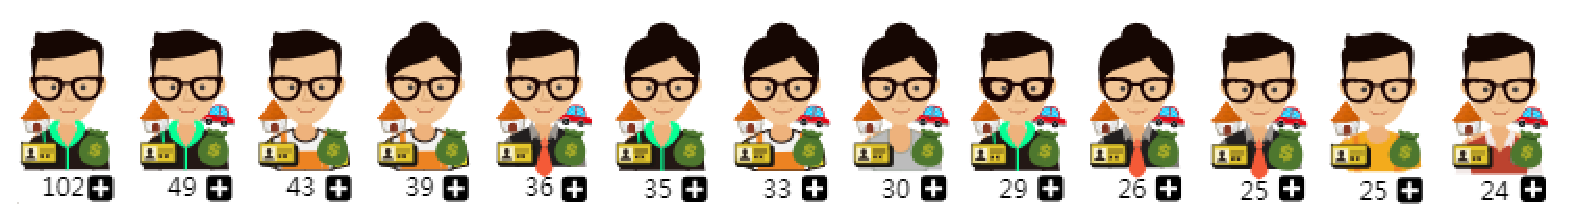
\includegraphics{pictures/case111.eps}}}\hspace{5pt}
\subfigure[The underclass.]{
\resizebox*{4.4cm}{!}{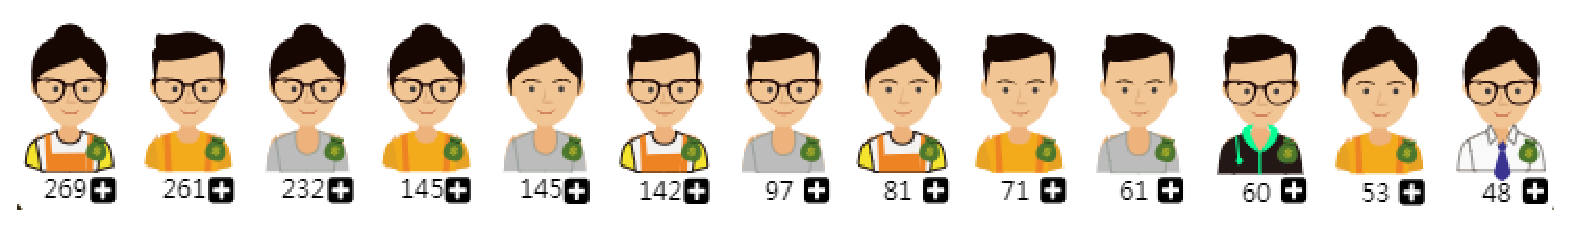
\includegraphics{pictures/case112.eps}}}\hspace{5pt}
\subfigure[New rich.]{
\resizebox*{4.4cm}{!}{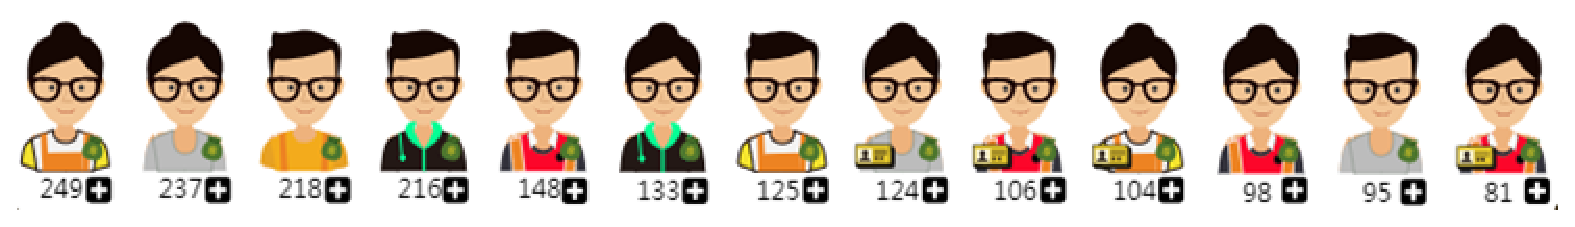
\includegraphics{pictures/case113.eps}}}\hspace{5pt}
\subfigure[Antizen.]{
\resizebox*{4.4cm}{!}{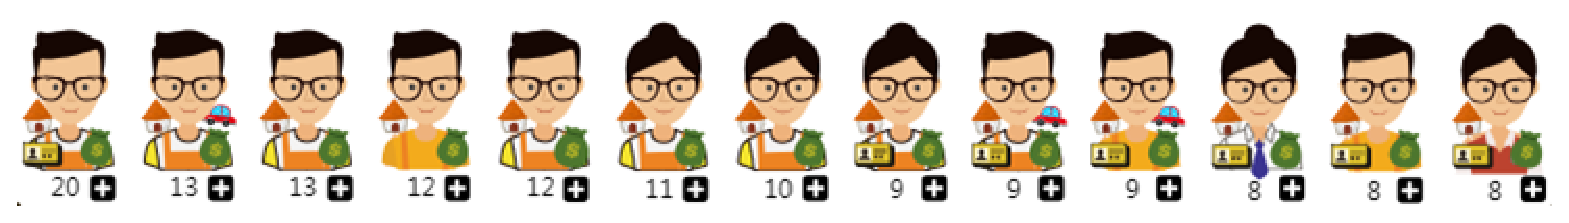
\includegraphics{pictures/case114.eps}}}\hspace{5pt}
\caption{XXX of different groups.}
\label{case11}
\end{figure}


\begin{figure}
\centering
\subfigure[Top aristocracy.]{
\resizebox*{4.4cm}{!}{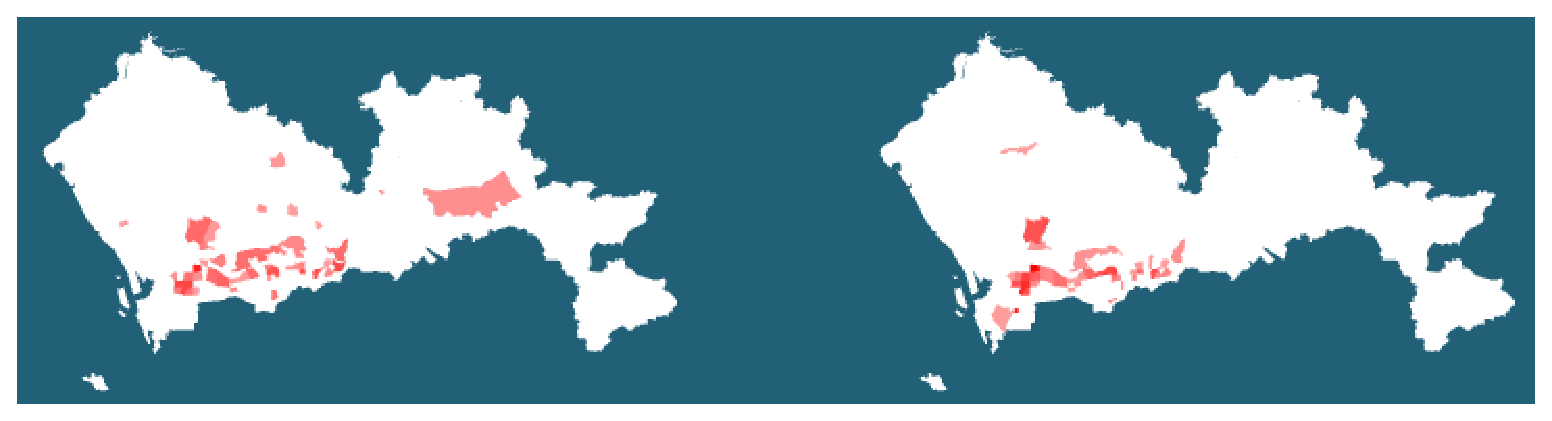
\includegraphics{pictures/case121.eps}}}\hspace{5pt}
\subfigure[The underclass.]{
\resizebox*{4.4cm}{!}{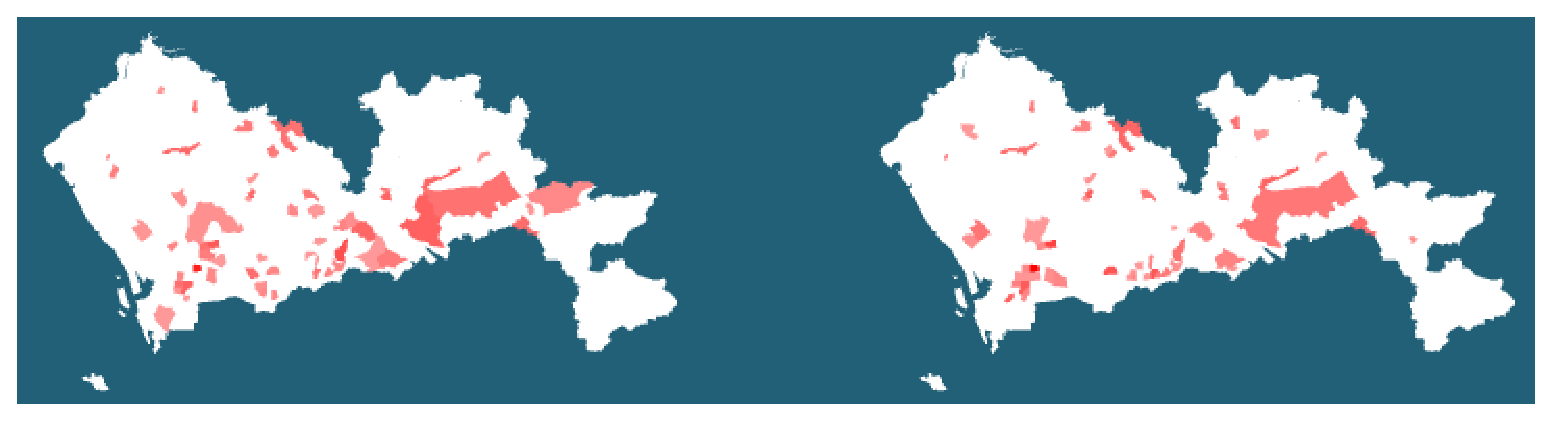
\includegraphics{pictures/case122.eps}}}\hspace{5pt}
\subfigure[New rich.]{
\resizebox*{4.4cm}{!}{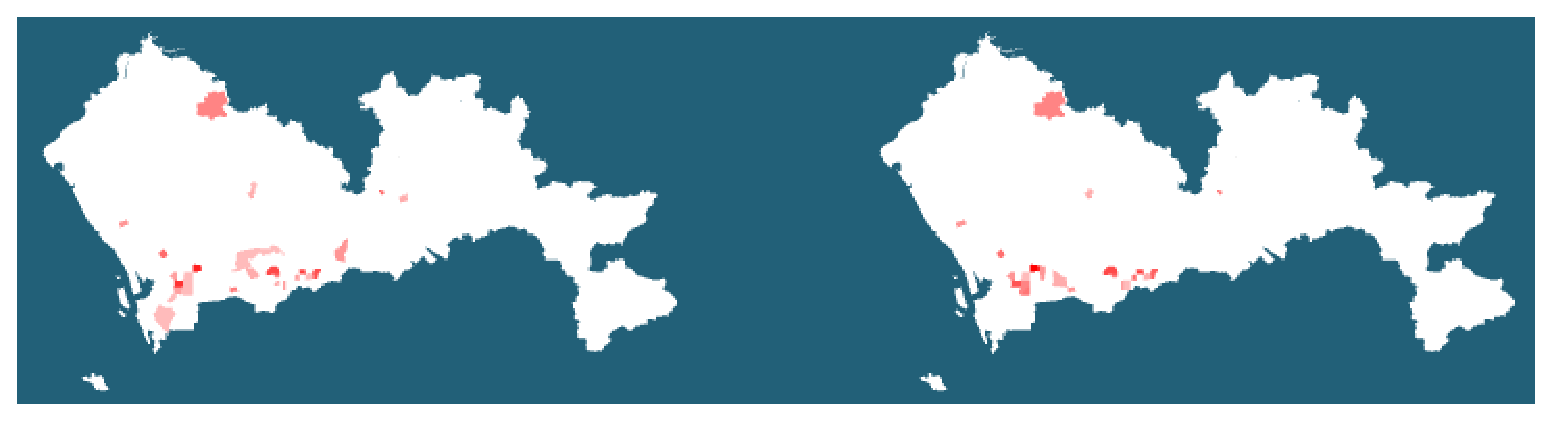
\includegraphics{pictures/case123.eps}}}\hspace{5pt}
\subfigure[Antizen.]{
\resizebox*{4.4cm}{!}{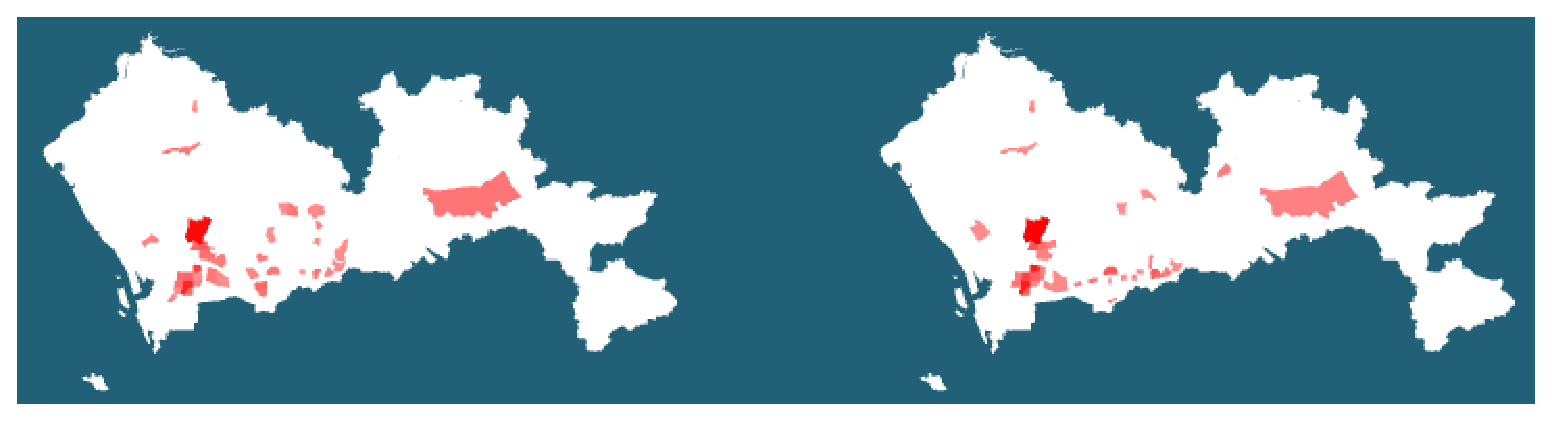
\includegraphics{pictures/case124.eps}}}\hspace{5pt}
\caption{Distributions of home and working space of different groups.}
\label{case12}
\end{figure}


\begin{figure}
\centering
\subfigure[Top aristocracy.]{
\resizebox*{4.4cm}{!}{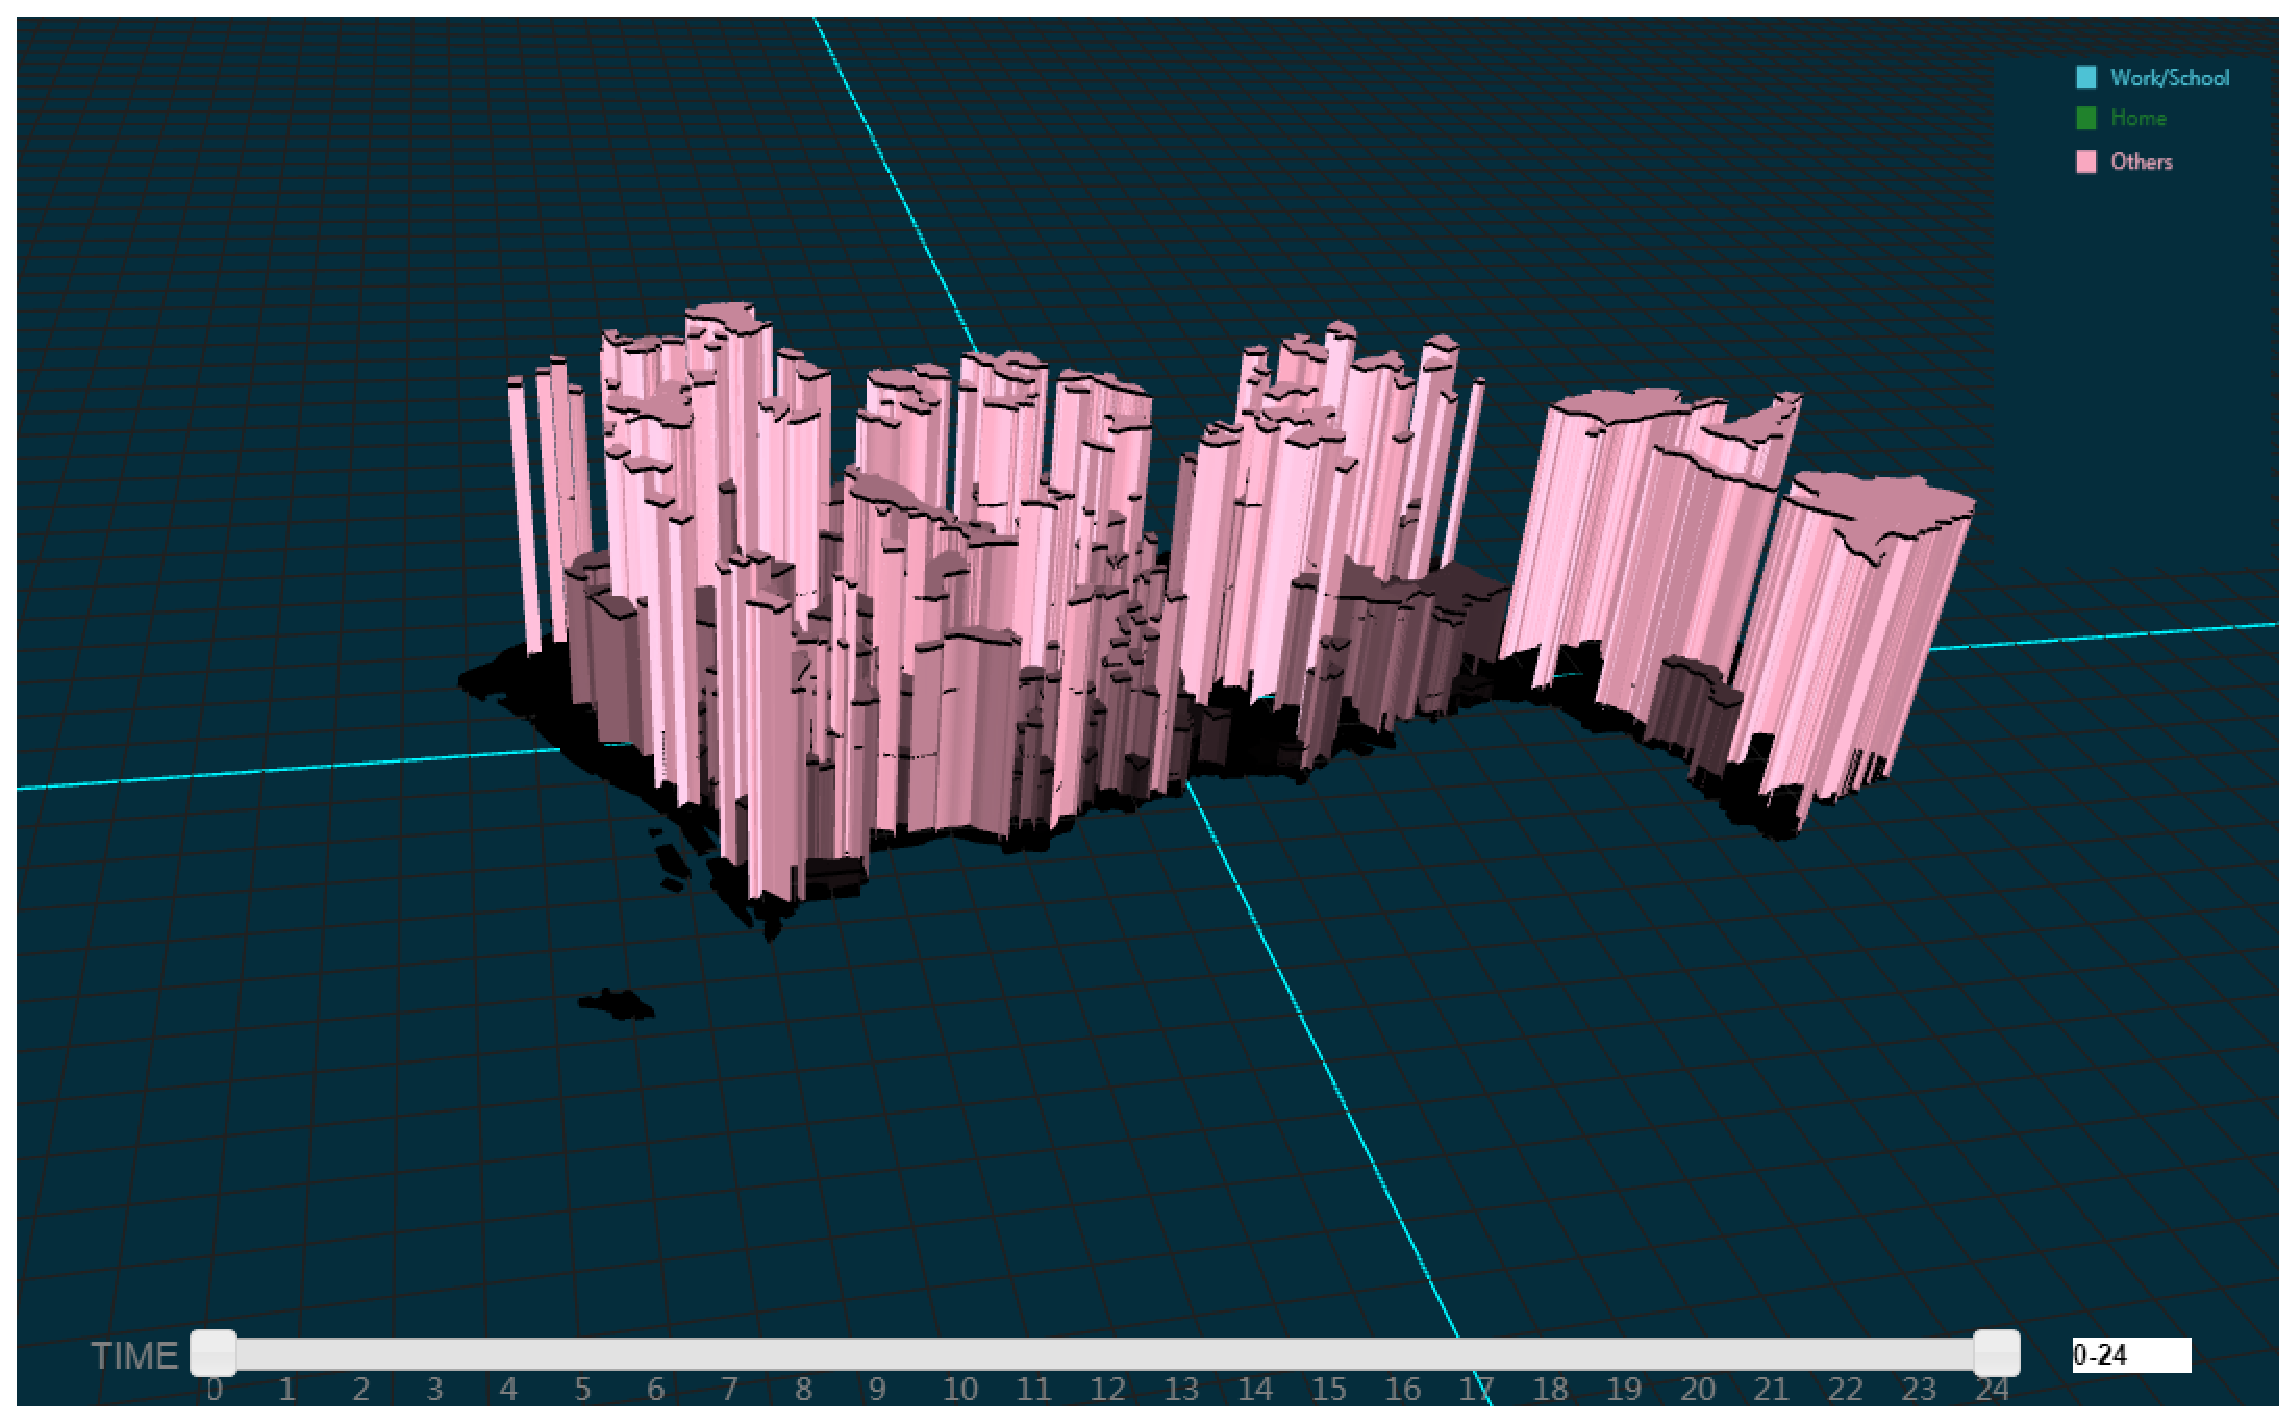
\includegraphics{pictures/case131.eps}}}\hspace{5pt}
\subfigure[The underclass.]{
\resizebox*{4.4cm}{!}{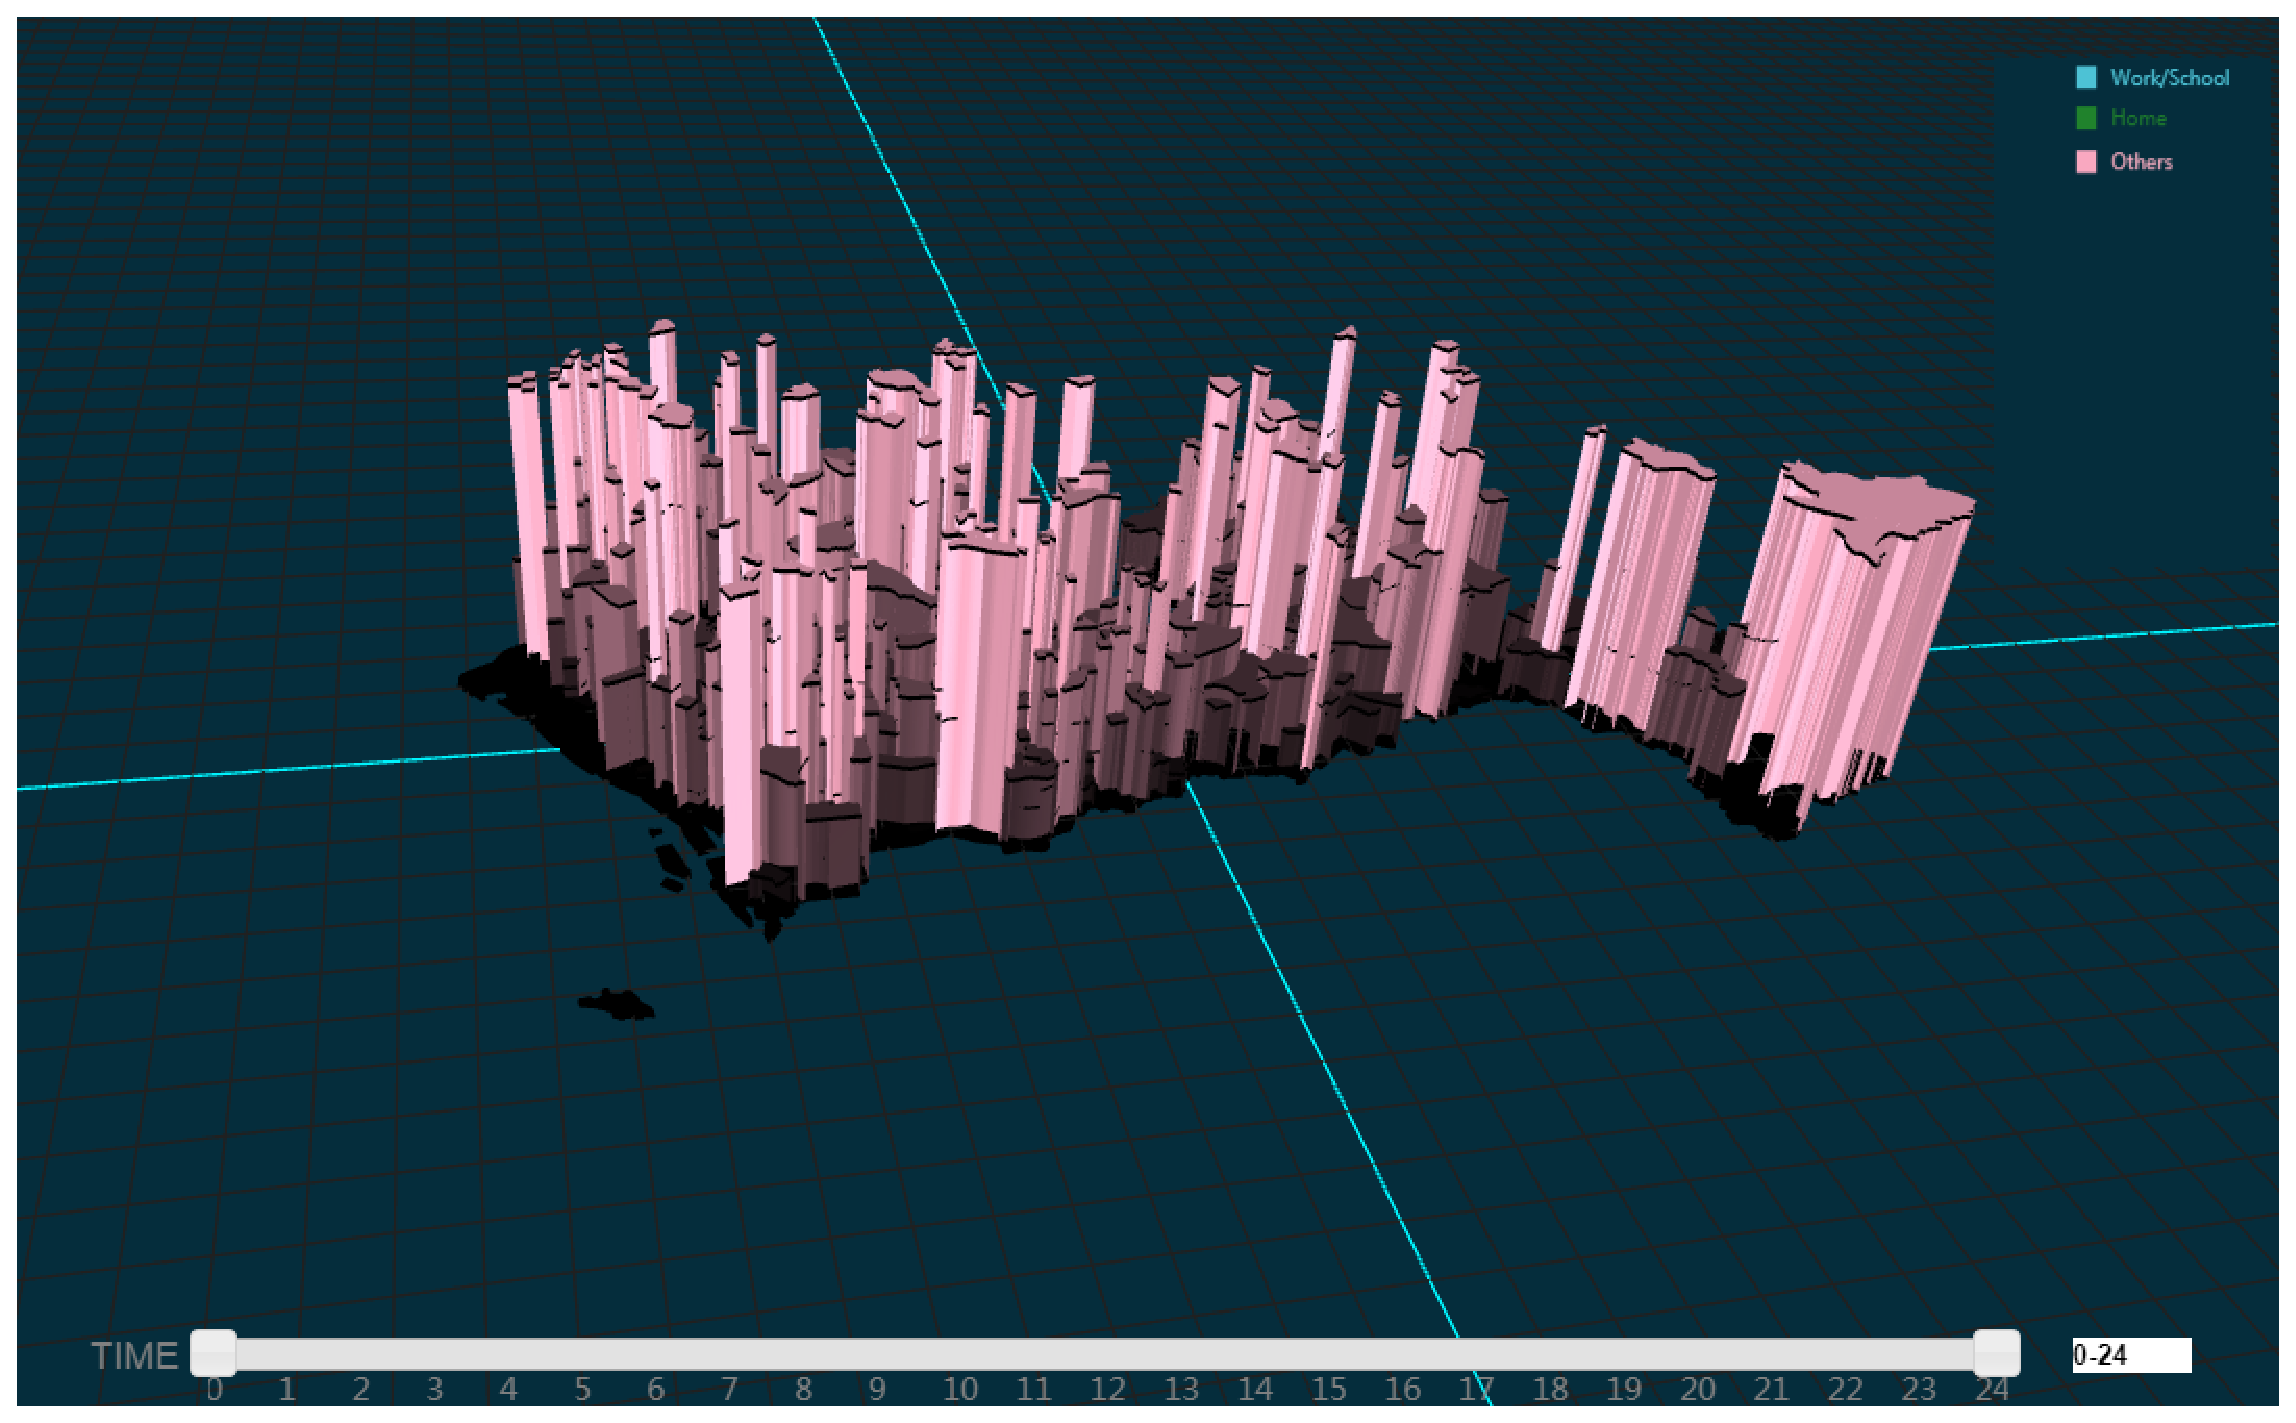
\includegraphics{pictures/case132.eps}}}\hspace{5pt}
\subfigure[New rich.]{
\resizebox*{4.4cm}{!}{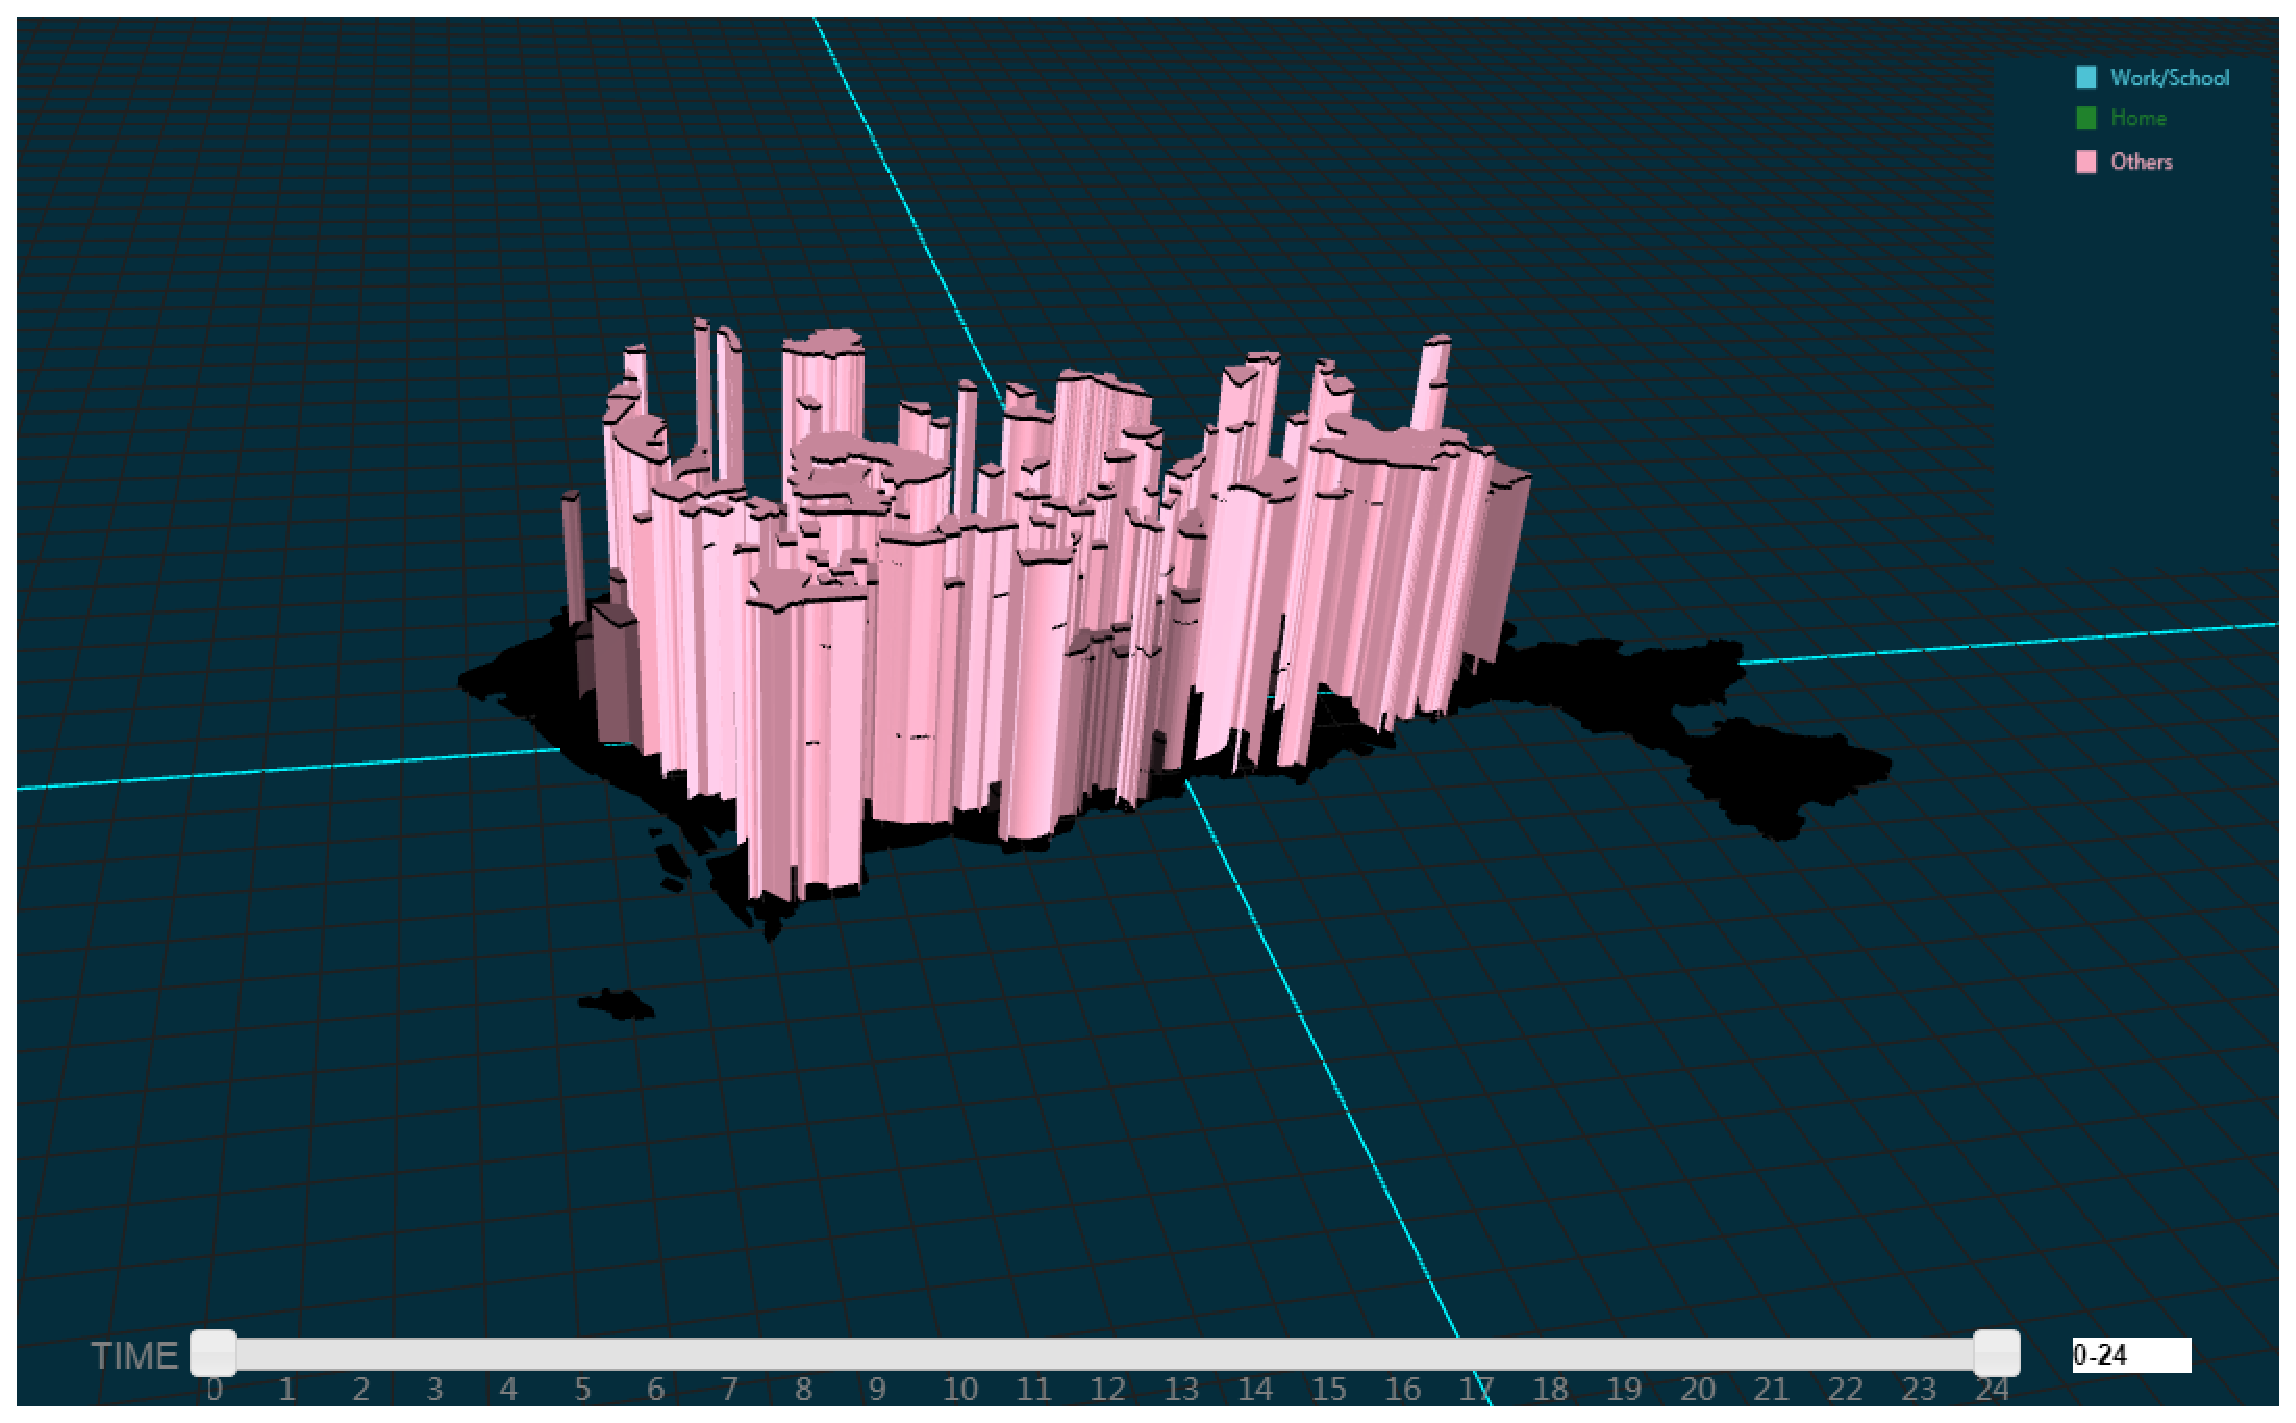
\includegraphics{pictures/case133.eps}}}\hspace{5pt}
\subfigure[Antizen.]{
\resizebox*{4.4cm}{!}{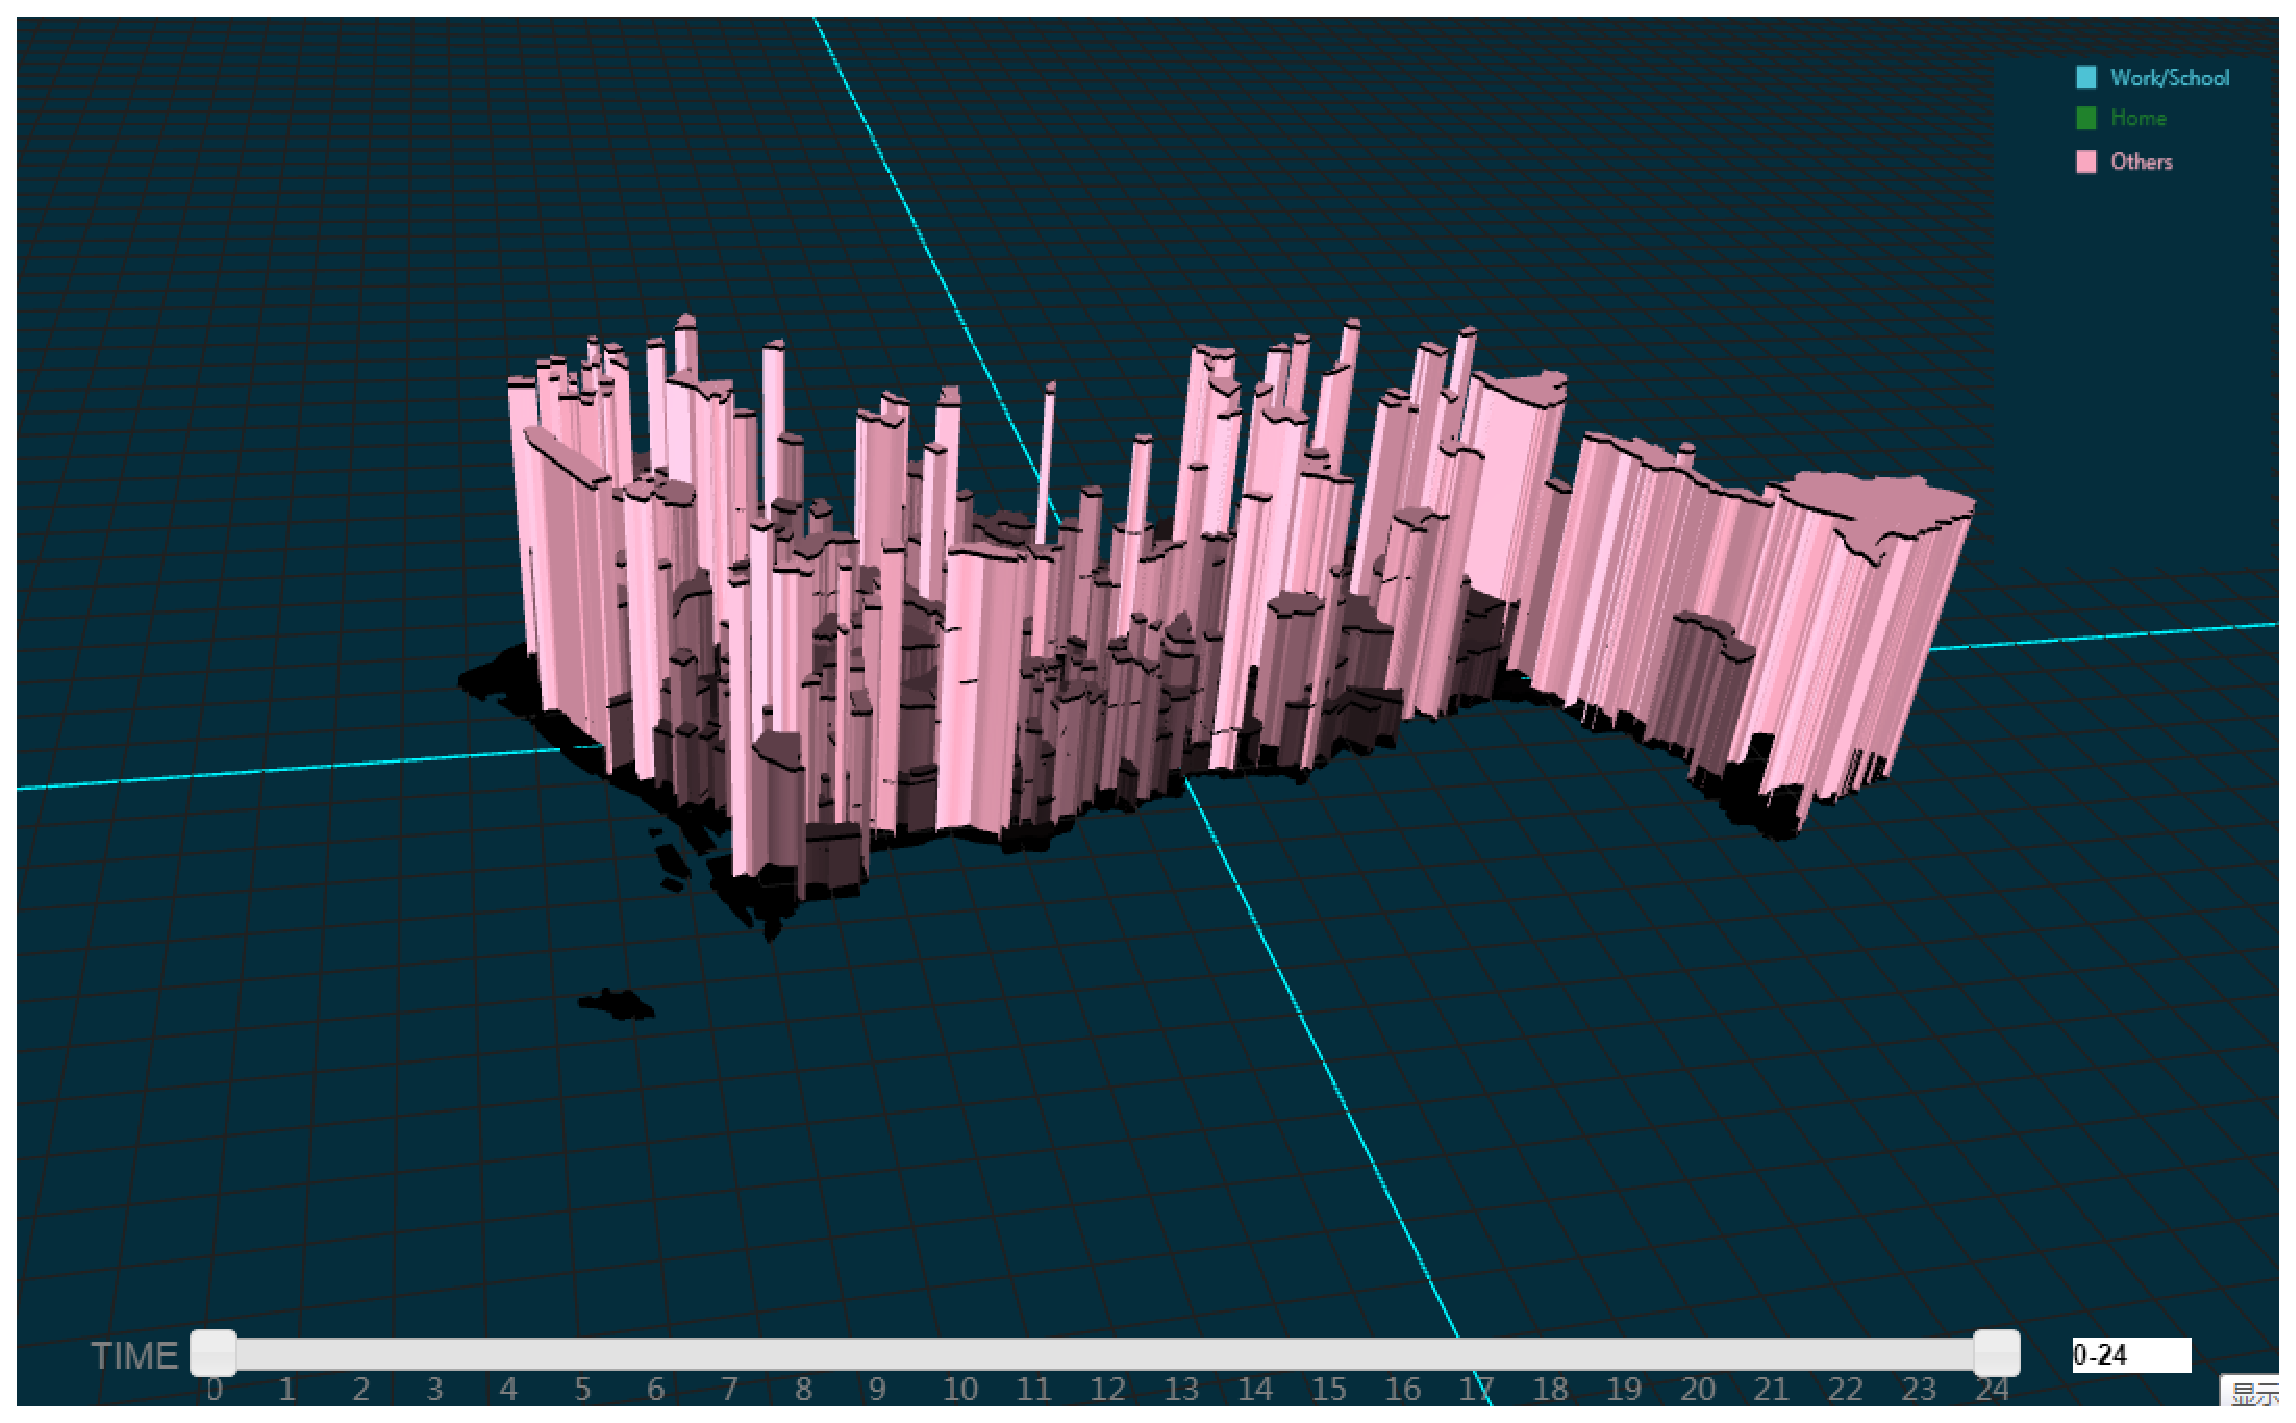
\includegraphics{pictures/case134.eps}}}\hspace{5pt}
\caption{Distribution of ``not essential" activity of different groups.}
\label{case13}
\end{figure}
The most important factors in \textit{Folding Beijing} are wealth and social status. In this case, we select ``income" and ``education" to express the two factors to explore citizens' mobility and city usage.

We deem persons earning more than 300,000 yuan a year are in rich group, while less than 100,000 yuan are in poor group. Persons with undergraduate diploma belong to high education group. So, there are four groups formed. The first one is ``top aristocracy" with high income and education level. Opposite of them, ``the underclass" have lowest income and little education. Group ``new rich" collects people who are rich but have less education. ``Antizen" is a new word to describe people have good education but earn little, which is the fourth group.

Fig. \ref{case11} shows the top 13 persons' images in each group. Except for income and education, other social features describe every group in different ways. As shown, nearly all of ``top aristocracy" are locals owing house and car. On the contrary, ``the underclass" do not owe local residence, neither the house and car. ``New rich" can afford house. Most of them are in service industry.

To understand how citizens live in the city, there are two crucial aspects to be known: during the night where they sleep, and where do they go during the daytime.
We divide daytime mobility activities into ``essential activity" and ``no essential activity" two categories to capture movement patterns. ``Essential activity" is made up with ``go to work", ``go to school" and ``go back home". Movements with other purposes are ``not essential". People do these movement activities due to their personal willingness and living patterns. Therefore, ``home location", ``working location" and ``not essential" activity space outline one's living space. Our system meets this requirement.

Fig. \ref{case12} shows examples of living space of the four groups. Fig. \ref{case12}(a) and Fig. \ref{case12}(b) show the distributions of home and working space. These two distributions are similar in four groups. ``Top aristocracy" and ``new rich" live concentrated in downtown area of Shenzhen, where the living cost is higher, especially the housing cost. ``The underclass" distribute dispersively all over the whole city. Compared to the rich, the outer space are prefered because of the lower living cost. Lots of ``antizen" live in Nanshan District. There are many universities and high-tech industrial parks are located in Nanshan which attracts good educated persons. The distribution of ``not essential activity" is shown in Fig. \ref{case13}. From the dimension of space, ``new rich" prefer to live in the west of the city. They do not go south east in most times. Other three groups reach the whole city. The height of the bar stands for the percentage of ``not essential activity" in the whole activities. Higher height means that the group has more willingness and cost more time in ``not essential activity", while lower height means more time on work. Comparing four groups, it can be seen that the poor spend more time on work, especially ``the underclass". Working percentage is really small in group ``new rich". They have diverse lives because they do many other things except for working.


\subsection{Case 2: Home-work Distance}
\begin{figure}
\centering
\subfigure[Group of people whose income more than 500,000yuan per year.]{
\resizebox*{4.4cm}{!}{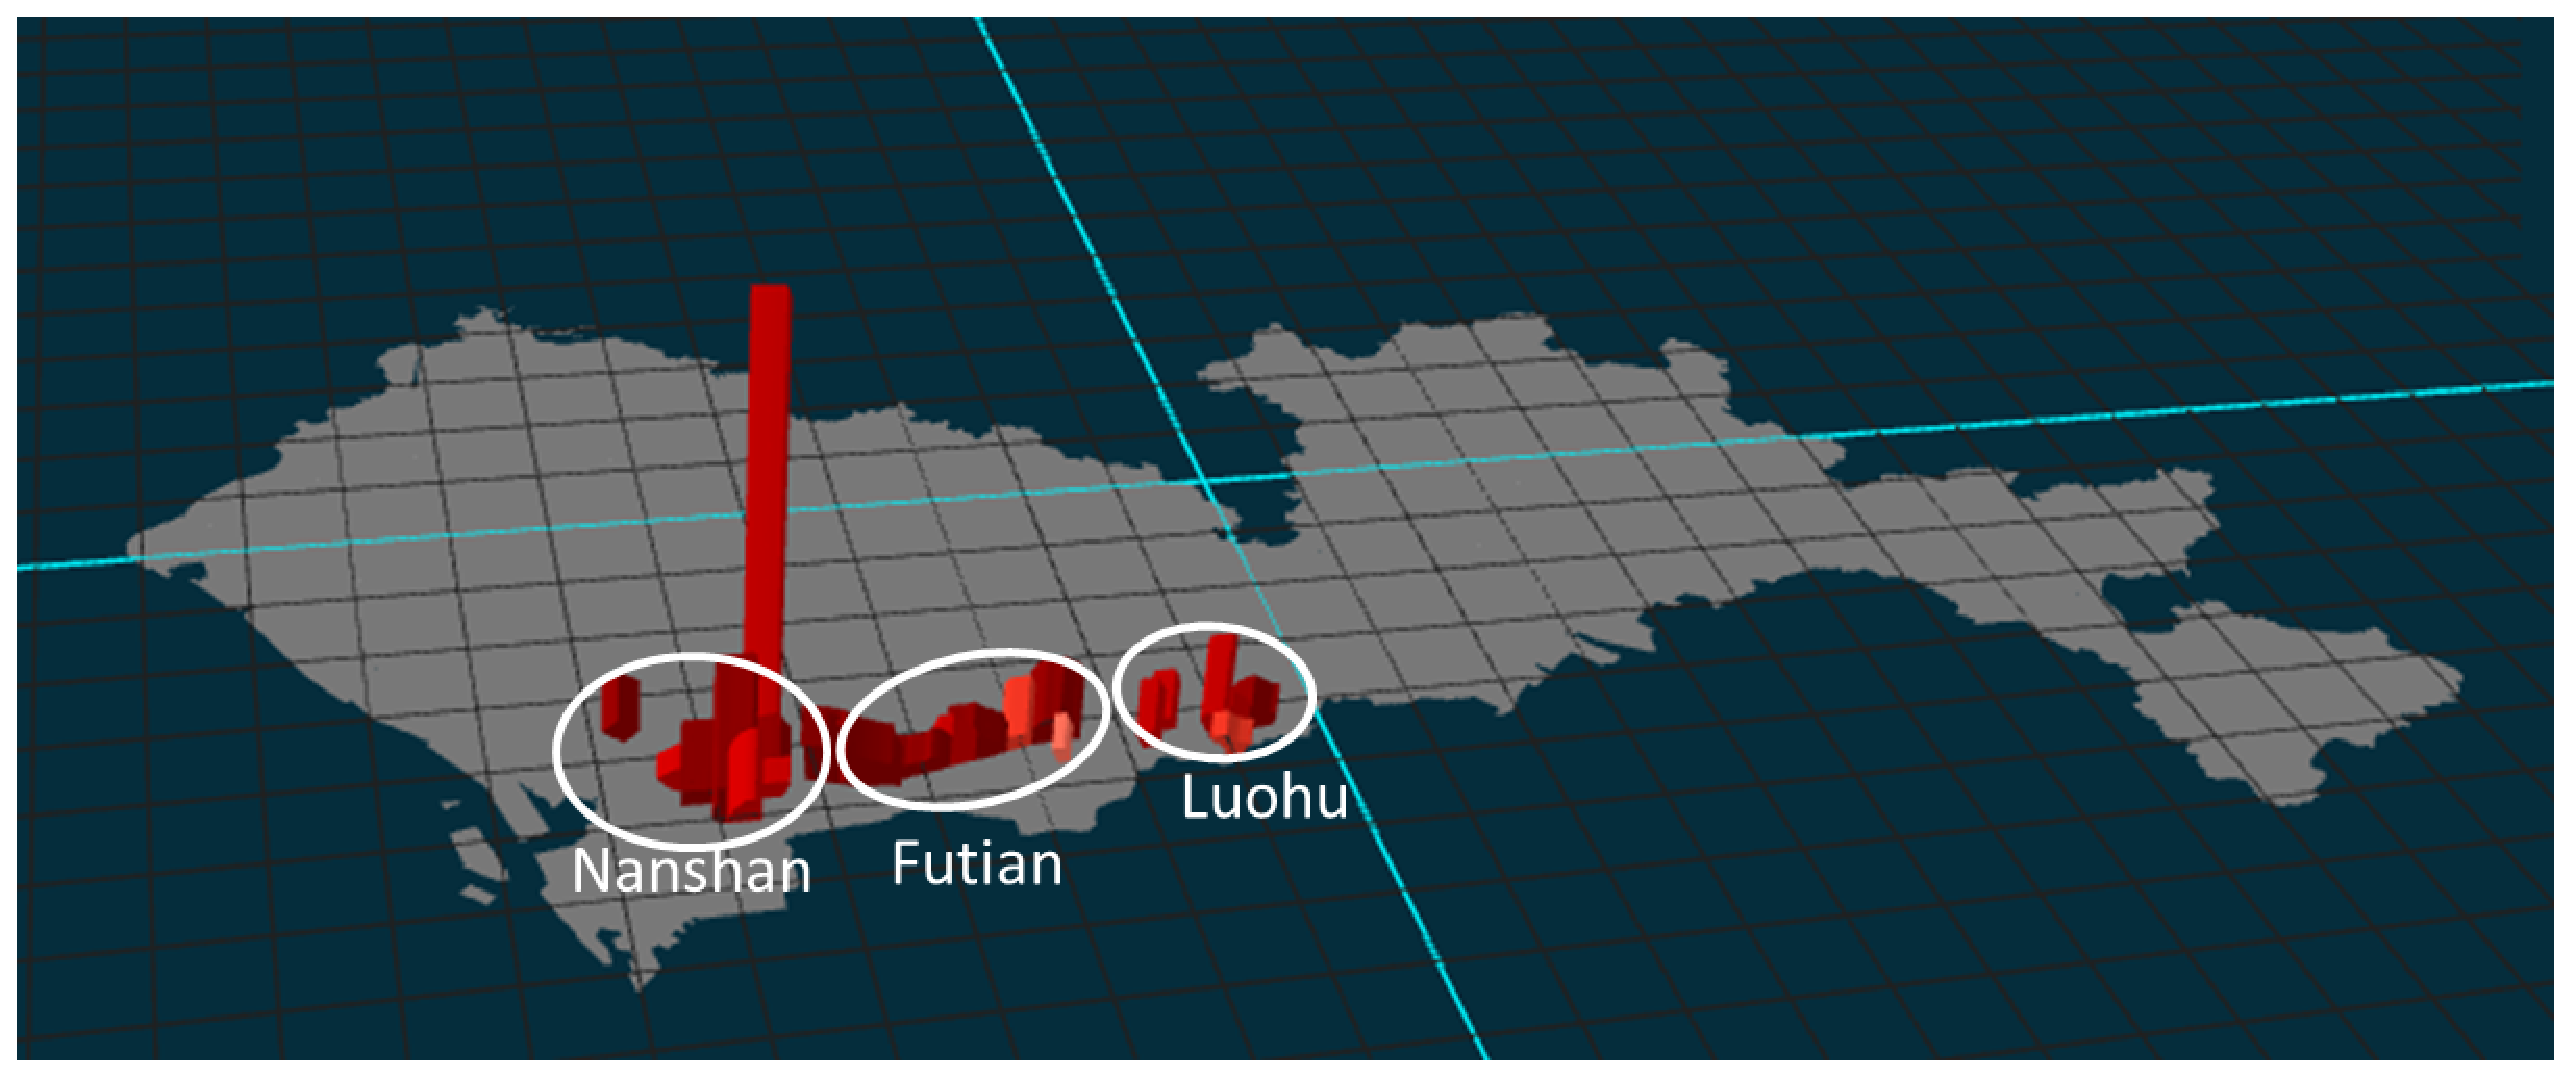
\includegraphics{pictures/case21.eps}}}\hspace{5pt}
\subfigure[Group of people whose income between 200,000 yuan to 300,000 yuan per year.]{
\resizebox*{4.4cm}{!}{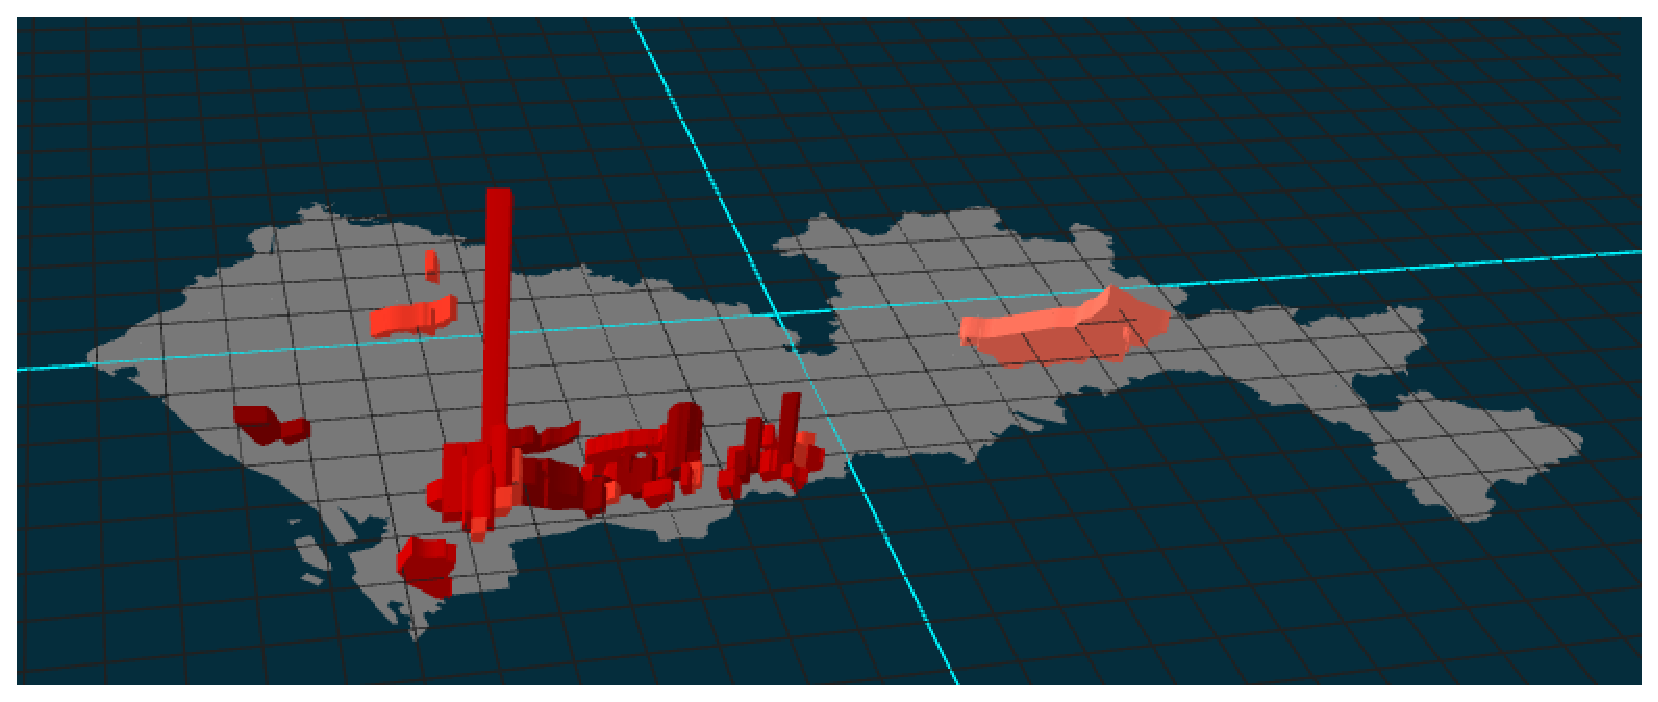
\includegraphics{pictures/case22.eps}}}\hspace{5pt}
\subfigure[Group of people whose income less than 100,000yuan per year.]{
\resizebox*{4.4cm}{!}{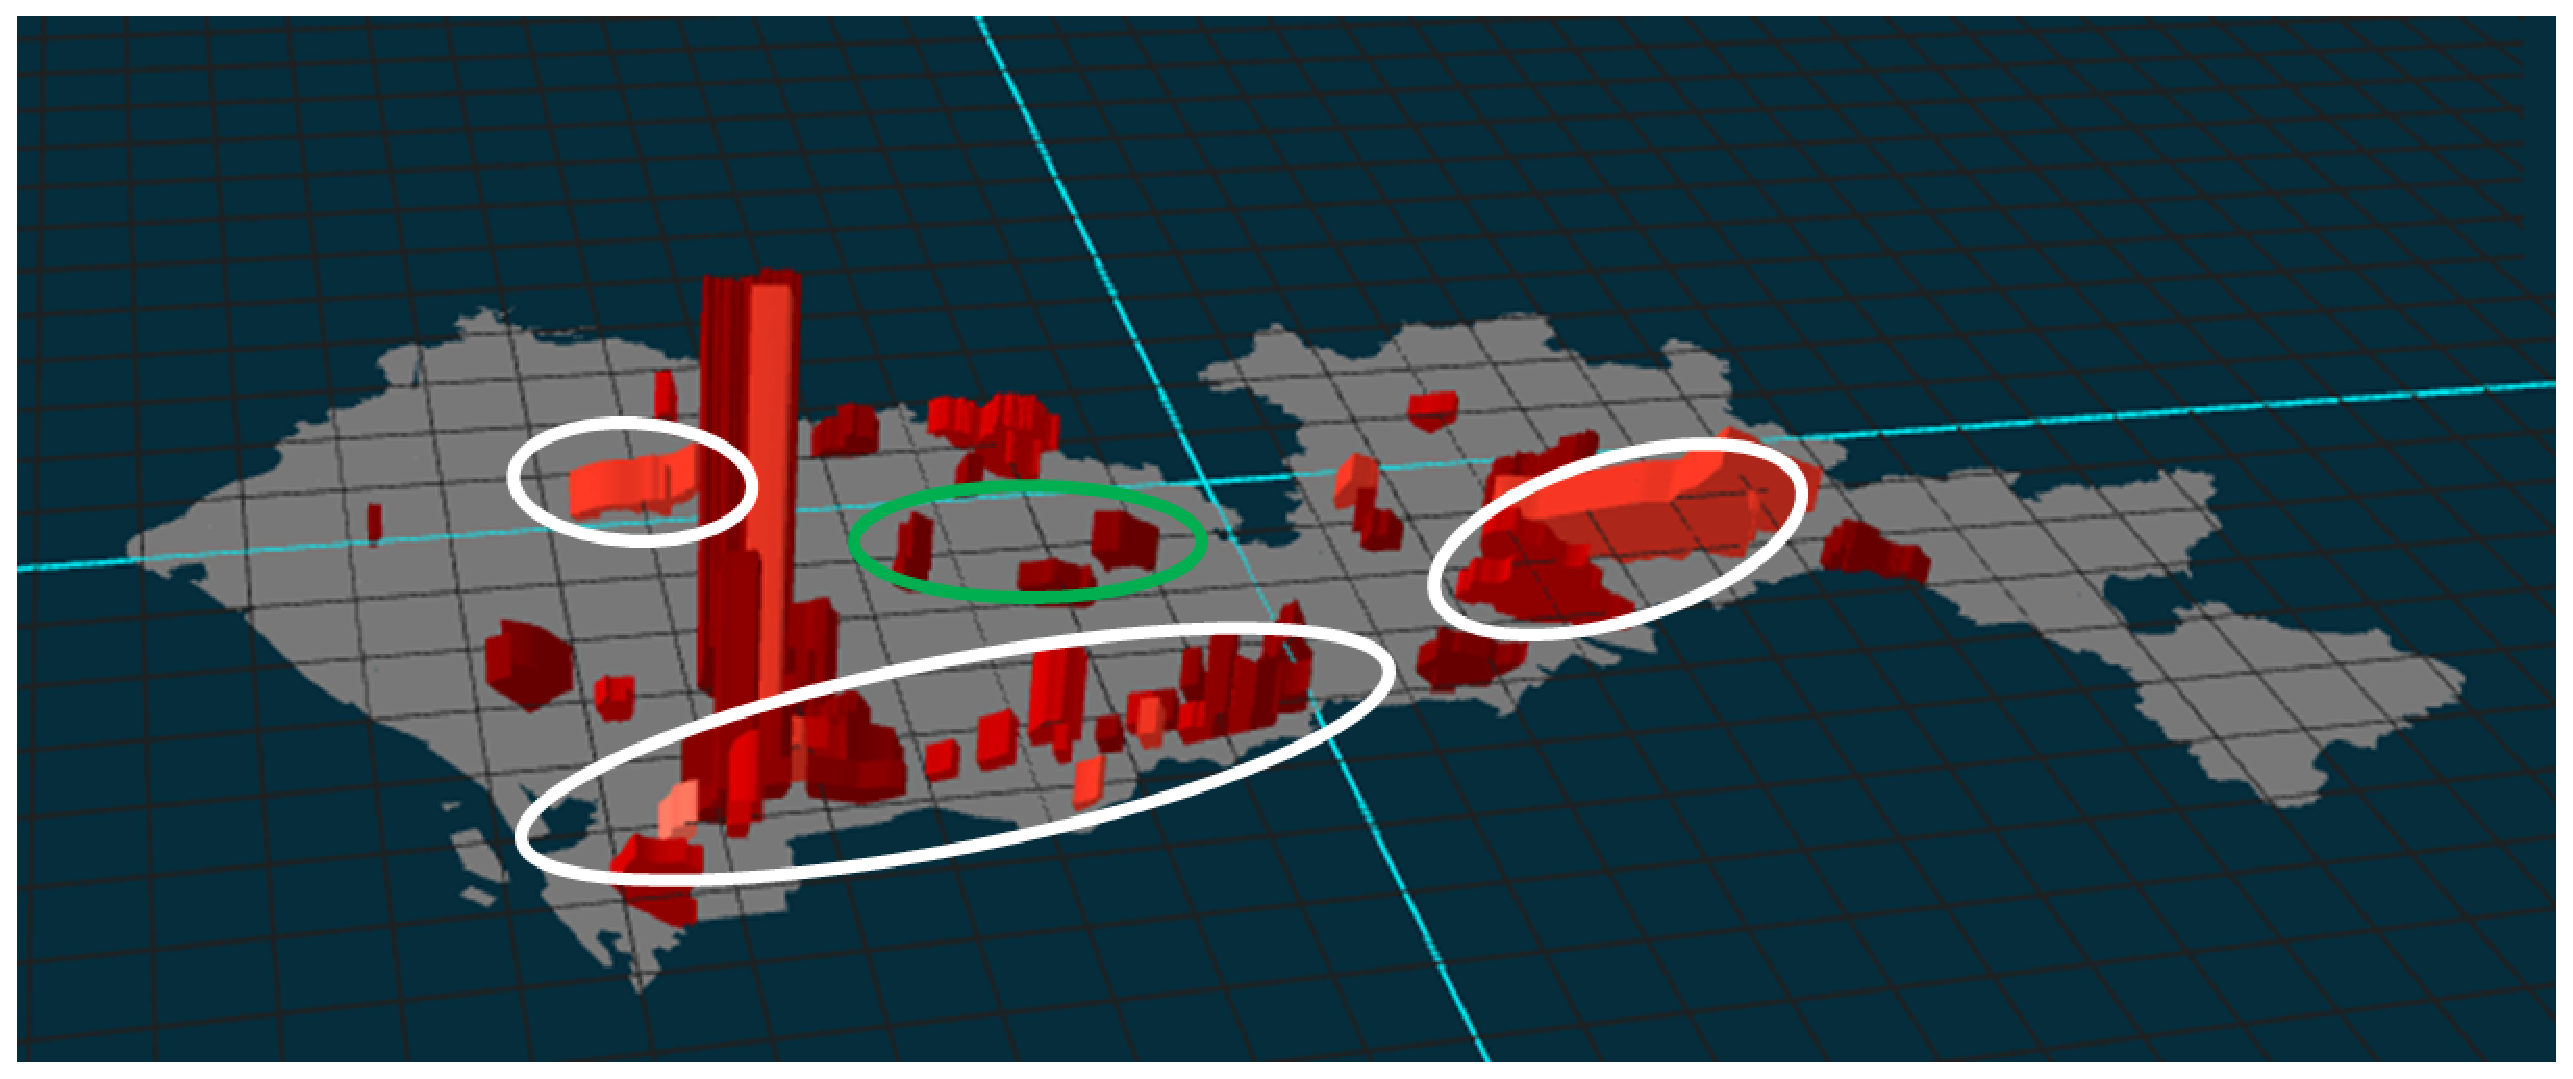
\includegraphics{pictures/case23.eps}}}\hspace{5pt}
\subfigure[Group of people who owe house.]{
\resizebox*{4.4cm}{!}{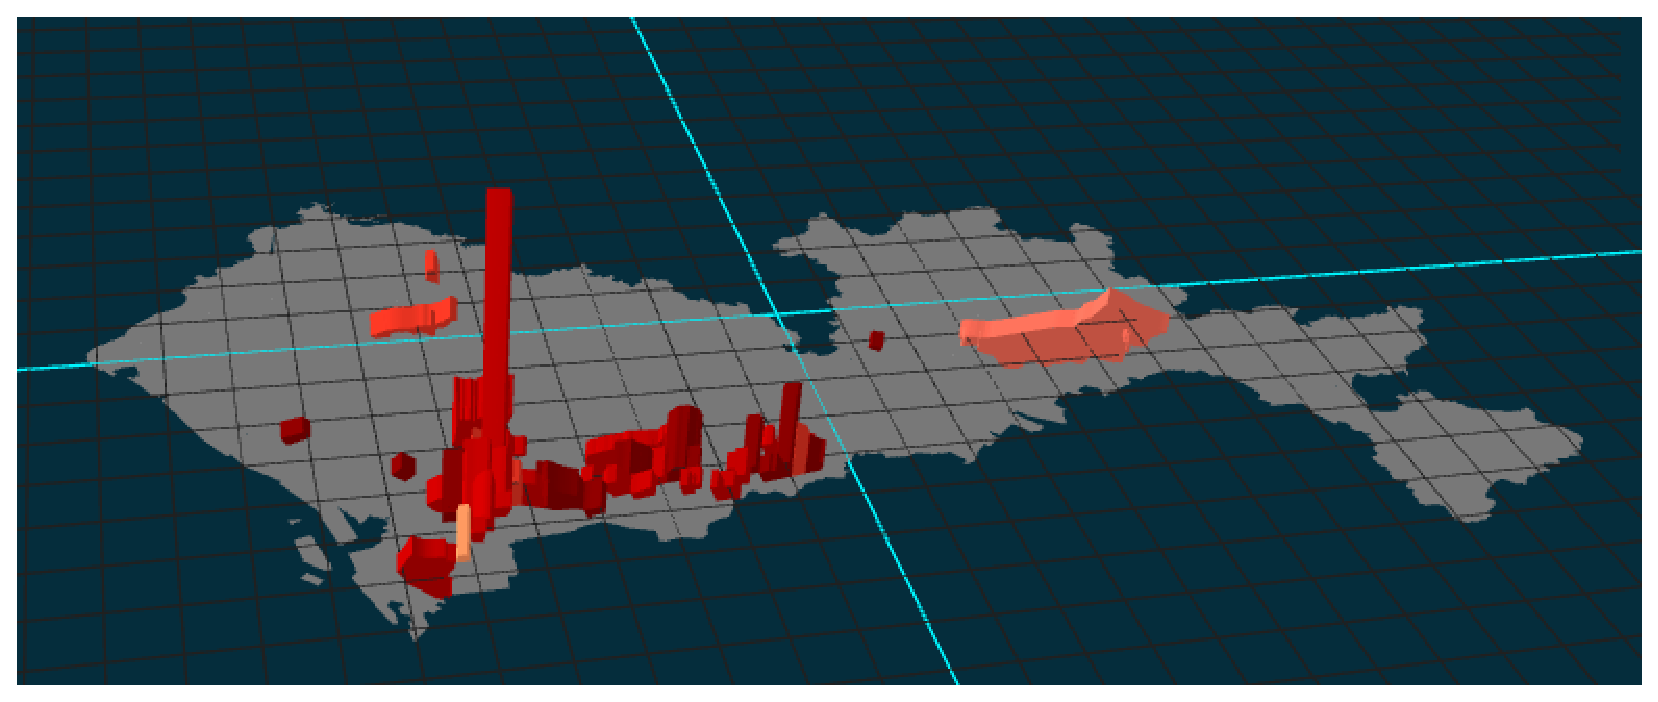
\includegraphics{pictures/case24.eps}}}\hspace{5pt}
\subfigure[Group of people who rent house.]{
\resizebox*{4.4cm}{!}{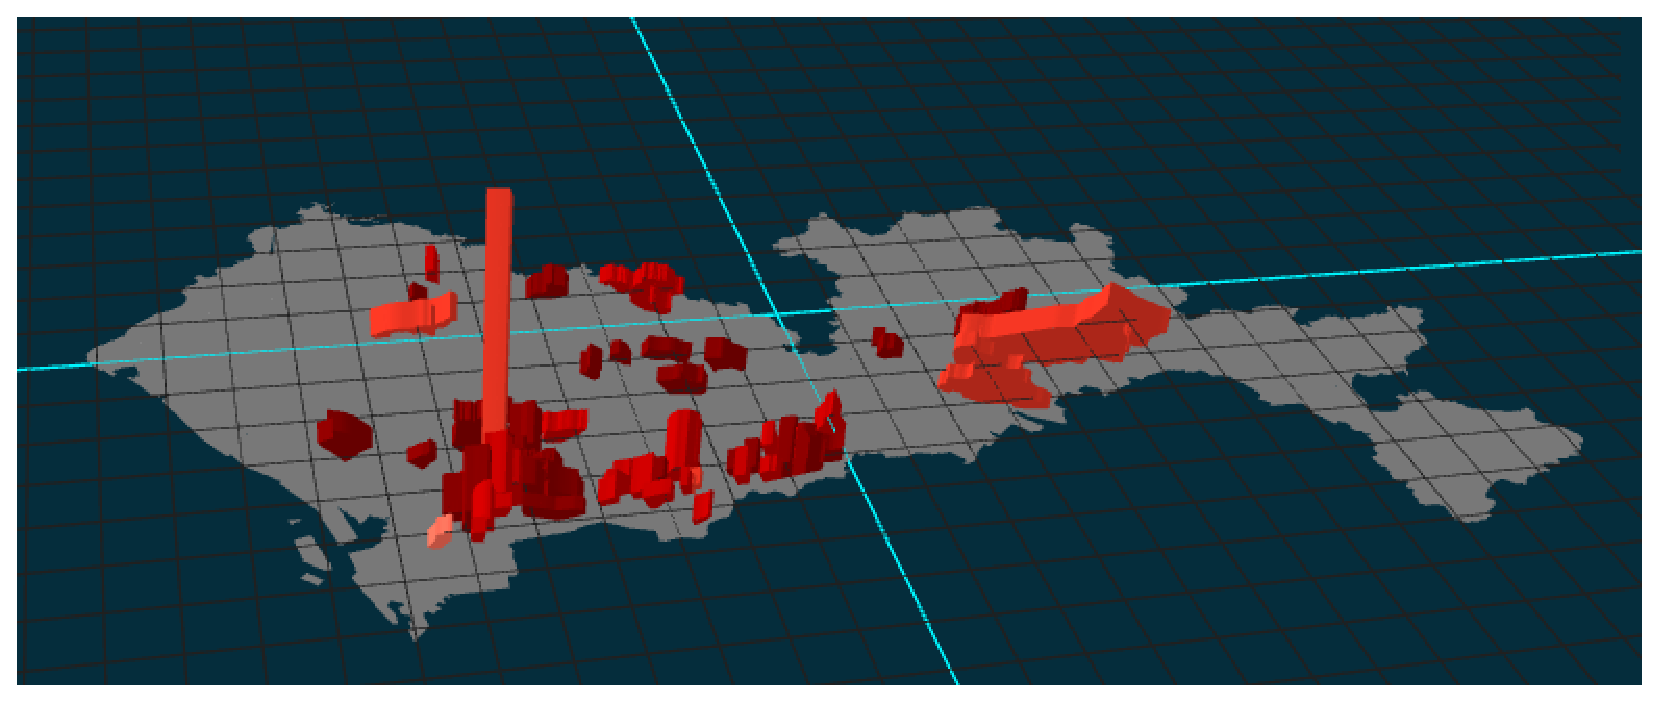
\includegraphics{pictures/case25.eps}}}\hspace{5pt}
\caption{Home-work distances of different groups.}
\label{case2}
\end{figure}
Home-work space and commuting behavior is an important concept in economics, geography and sociology. It is influenced by many factors like transportation, housing, land using, etc. Understanding it helps know how city functions for a better planning. In this case, we use a graph of ``working space and commuting distance" to demonstrate our system's help in movement behavior understanding.

We use ``income" and ``have house" to distinguish citizens and learn their home-work distance. Fig. \ref{case2} shows examples of five groups. Fig. \ref{case2}(a), Fig. \ref{case2}(b) and Fig. \ref{case2}(c) are formed according to ``income". They are ``more than 500,000 yuan", ``200,000 to 300,000 yuan" and ``less than 100,000 yuan" levels separately. Fig. \ref{case2}(d) and Fig. \ref{case2}(e) are for group of people ``owing house" and ``rent house".

The height of the bar stands for working frequency of the TAZ. From the figure, it is seen that the working locations are mainly in three areas which are circled in white in Fig. \ref{case2}(c). Space in green circle is another hot working area which only are preferred by the poor.

The color of the bar stands for home-work distance of people working in the TAZ. On the whole, home-work distance is short in Shenzhen for most of the TAZs with different groups have darker color, especially in downtown. When focusing on downtown area, it is seen that there are differences between Futian District with the other two. By comparing three groups distinguished by income, it takes more time to work in Futian District with the decrease of the income. Meanwhile, the opposite is true in others. In combination with Fig. \ref{case2}(d) and Fig. \ref{case2}(e), we find that Nanshan District and Luohu District belongs to all but Futian District belongs to the rich. The poor could rent house living in Nanshan and Luohu to enjoy short home-work distance. In Futian, only the rich working there have short home-work distance. There may be no much housing for rent.

